\documentclass[10pt]{beamer}

\usetheme[progressbar=frametitle]{metropolis}
\usepackage{appendixnumberbeamer}

\usepackage{booktabs}
\usepackage[scale=2]{ccicons}

\usepackage{pgfplots}
\usepgfplotslibrary{dateplot}

\usepackage{xspace}
\newcommand{\themename}{\textbf{\textsc{metropolis}}\xspace}

\title{YACRA - Yet Another Code Retrieval Approach}
\subtitle{Um estudo preliminar sobre o uso de uma arquitetura deep learning para seleção de respostas no problema de recuperação de código-fonte}
% \date{\today}
\date{}
\author{Marcelo de Rezende Martins\inst{1}, Marco Aurélio Gerosa\inst{2}}
\institute{\inst{1}Instituto de Pesquisas Tecnológicas
  (IPT) \and \inst{2}Northern Arizona University (NAU)}
% \titlegraphic{\hfill\includegraphics[height=1.5cm]{logo.pdf}}

\begin{document}

\maketitle

\begin{frame}{Índice}
  \setbeamertemplate{section in toc}[sections numbered]
  \tableofcontents%[hideallsubsections]
\end{frame}

\section[Introdução]{Introdução}

\begin{frame}[fragile]{Definição}

A tarefa do \textit{code retrieval} ou recuperação de trecho de código-fonte consiste em:
 
\emph{Dado uma descrição em linguagem natural, recuperar o trecho de código-fonte mais relevante, tal que os desenvolvedores possam encontrar rapidamente os trechos de código que atendam as suas necessidades. \cite{Chen-bi-variational-autoencoder:2018}}
 
\end{frame}
\begin{frame}[fragile]{Definição}
  \textbf{Code Retrieval}: Dada uma questão em linguagem natural $Q$, um modelo $F_{r}$ irá aprender a recuperar o trecho de código-fonte $C^{*} \in \mathbb{C}$ com a maior pontuação \cite{yao-2018}:

\begin{equation}\label{eq:code-retrieval}
C^{*} = \underset{C \in \mathbb{C}}{argmax}\text{ } F_{r}(Q , C)
\end{equation}
  
\end{frame}

\section{Abordagem}

\begin{frame}{Hipótese inicial}
	\textbf{Hipótese inicial:} \emph{software é uma forma de comunicação humana e tem propriedades estatísticas similares a corpora de linguagem natural \cite{Allamanis:2018:SML}}
\end{frame}

\begin{frame}{Joint embedding}
	Seja $\mathbb{Q}$ o conjunto formado pelas questões e $\mathbb{C}$ o conjunto composto por trechos de código-fonte \cite{Gu-deep-code-search:2018}:
	
    \begin{equation}
        \mathbb{C} \xrightarrow{\mathbb{E}_{c}} \mathbb{V}_{c} \rightarrow \mathbb{J}(\mathbb{V}_{c}, \mathbb{V}_{q}) \leftarrow \mathbb{V}_{q} \xleftarrow{\mathbb{E}_{q}} \mathbb{Q}
    \end{equation}
\end{frame}


\begin{frame}{Forma de aprendizagem}
	Função de perda \textit{hinge} \cite{tan-lstm-qa, Gu-deep-code-search:2018}:
	
    \begin{equation}
    L = max(0, m - \mathbb{J}(q_{i}, c_{i}^{+}) + \mathbb{J}(q_{i}, c_{i}^{-}))   
    \end{equation}
\end{frame}





\begin{frame}{Arquitetura}
	\begin{figure}[h]
    \centering
    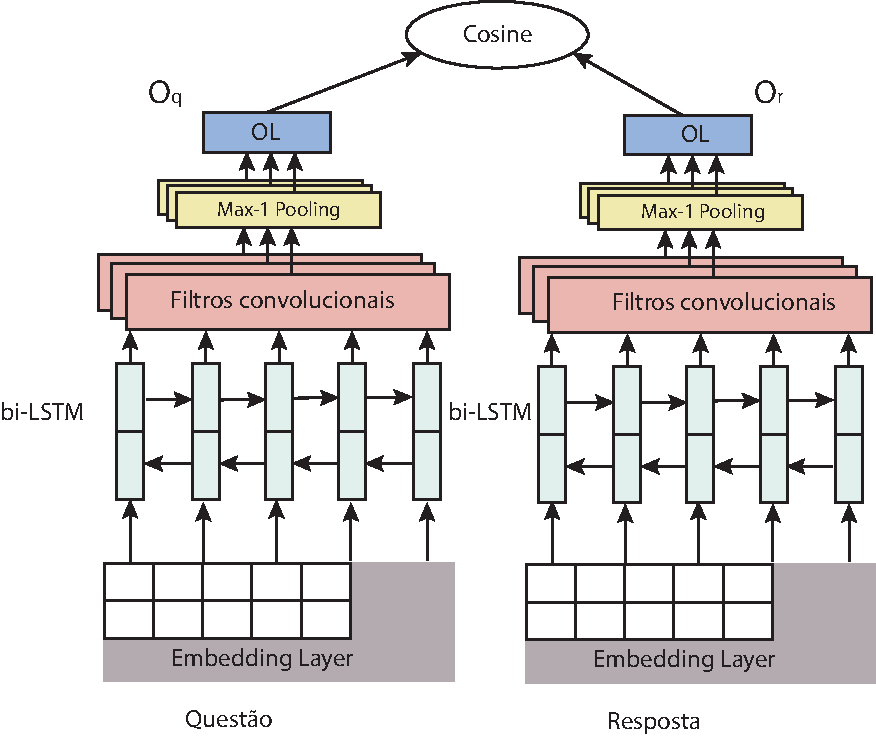
\includegraphics[width=0.7\textwidth]{ArquiteturaBiLSTM.pdf}
    \caption{Figura adaptada do \cite{tan-lstm-qa}.}
    \label{fig:arquitetura-bi-lstm}
\end{figure}
\end{frame}


\section{Experimento}

\begin{frame}[fragile]{Treinamento}
      \begin{table}[h]
\centering
\begin{tabular}{ p{3cm} r  }
 \hline
 \textbf{Amostras} & \textbf{Quantidade de $(q_{i}, c_{i}^{+})$}\\
 \hline
 Treinamento & $60.083$\\
 
 DEV & $1.085$ \\
 
 EVAL & $1.084$\\
 \hline
 \textbf{Total} & $\textbf{62.252}$\\
 \hline
\end{tabular}
\caption{Divisão das amostras para treinamento conforme os critérios adotados por \cite{iyer-etal-2016-summarizing}.}
\label{table:divisao-amostras}
\end{table}
\end{frame}

\begin{frame}{Font feature test}
  \begin{itemize}
    \item Regular
    \item \textit{Italic}
    \item \textsc{SmallCaps}
    \item \textbf{Bold}
    \item \textbf{\textit{Bold Italic}}
    \item \textbf{\textsc{Bold SmallCaps}}
    \item \texttt{Monospace}
    \item \texttt{\textit{Monospace Italic}}
    \item \texttt{\textbf{Monospace Bold}}
    \item \texttt{\textbf{\textit{Monospace Bold Italic}}}
  \end{itemize}
\end{frame}

\begin{frame}{Lists}
  \begin{columns}[T,onlytextwidth]
    \column{0.33\textwidth}
      Items
      \begin{itemize}
        \item Milk \item Eggs \item Potatos
      \end{itemize}

    \column{0.33\textwidth}
      Enumerations
      \begin{enumerate}
        \item First, \item Second and \item Last.
      \end{enumerate}

    \column{0.33\textwidth}
      Descriptions
      \begin{description}
        \item[PowerPoint] Meeh. \item[Beamer] Yeeeha.
      \end{description}
  \end{columns}
\end{frame}
\begin{frame}{Animation}
  \begin{itemize}[<+- | alert@+>]
    \item \alert<4>{This is\only<4>{ really} important}
    \item Now this
    \item And now this
  \end{itemize}
\end{frame}
\begin{frame}{Figures}
  \begin{figure}
    \newcounter{density}
    \setcounter{density}{20}
    \begin{tikzpicture}
      \def\couleur{alerted text.fg}
      \path[coordinate] (0,0)  coordinate(A)
                  ++( 90:5cm) coordinate(B)
                  ++(0:5cm) coordinate(C)
                  ++(-90:5cm) coordinate(D);
      \draw[fill=\couleur!\thedensity] (A) -- (B) -- (C) --(D) -- cycle;
      \foreach \x in {1,...,40}{%
          \pgfmathsetcounter{density}{\thedensity+20}
          \setcounter{density}{\thedensity}
          \path[coordinate] coordinate(X) at (A){};
          \path[coordinate] (A) -- (B) coordinate[pos=.10](A)
                              -- (C) coordinate[pos=.10](B)
                              -- (D) coordinate[pos=.10](C)
                              -- (X) coordinate[pos=.10](D);
          \draw[fill=\couleur!\thedensity] (A)--(B)--(C)-- (D) -- cycle;
      }
    \end{tikzpicture}
    \caption{Rotated square from
    \href{http://www.texample.net/tikz/examples/rotated-polygons/}{texample.net}.}
  \end{figure}
\end{frame}
\begin{frame}{Tables}
  \begin{table}
    \caption{Largest cities in the world (source: Wikipedia)}
    \begin{tabular}{lr}
      \toprule
      City & Population\\
      \midrule
      Mexico City & 20,116,842\\
      Shanghai & 19,210,000\\
      Peking & 15,796,450\\
      Istanbul & 14,160,467\\
      \bottomrule
    \end{tabular}
  \end{table}
\end{frame}
\begin{frame}{Blocks}
  Three different block environments are pre-defined and may be styled with an
  optional background color.

  \begin{columns}[T,onlytextwidth]
    \column{0.5\textwidth}
      \begin{block}{Default}
        Block content.
      \end{block}

      \begin{alertblock}{Alert}
        Block content.
      \end{alertblock}

      \begin{exampleblock}{Example}
        Block content.
      \end{exampleblock}

    \column{0.5\textwidth}

      \metroset{block=fill}

      \begin{block}{Default}
        Block content.
      \end{block}

      \begin{alertblock}{Alert}
        Block content.
      \end{alertblock}

      \begin{exampleblock}{Example}
        Block content.
      \end{exampleblock}

  \end{columns}
\end{frame}
\begin{frame}{Math}
  \begin{equation*}
    e = \lim_{n\to \infty} \left(1 + \frac{1}{n}\right)^n
  \end{equation*}
\end{frame}
\begin{frame}{Line plots}
  \begin{figure}
    \begin{tikzpicture}
      \begin{axis}[
        mlineplot,
        width=0.9\textwidth,
        height=6cm,
      ]

        \addplot {sin(deg(x))};
        \addplot+[samples=100] {sin(deg(2*x))};

      \end{axis}
    \end{tikzpicture}
  \end{figure}
\end{frame}
\begin{frame}{Bar charts}
  \begin{figure}
    \begin{tikzpicture}
      \begin{axis}[
        mbarplot,
        xlabel={Foo},
        ylabel={Bar},
        width=0.9\textwidth,
        height=6cm,
      ]

      \addplot plot coordinates {(1, 20) (2, 25) (3, 22.4) (4, 12.4)};
      \addplot plot coordinates {(1, 18) (2, 24) (3, 23.5) (4, 13.2)};
      \addplot plot coordinates {(1, 10) (2, 19) (3, 25) (4, 15.2)};

      \legend{lorem, ipsum, dolor}

      \end{axis}
    \end{tikzpicture}
  \end{figure}
\end{frame}
\begin{frame}{Quotes}
  \begin{quote}
    Veni, Vidi, Vici
  \end{quote}
\end{frame}

{%
\setbeamertemplate{frame footer}{My custom footer}
\begin{frame}[fragile]{Frame footer}
    \themename defines a custom beamer template to add a text to the footer. It can be set via
    \begin{verbatim}\setbeamertemplate{frame footer}{My custom footer}\end{verbatim}
\end{frame}
}

\begin{frame}{References}
  Some references to showcase [allowframebreaks] \cite{knuth92,ConcreteMath,Simpson,Er01,greenwade93}
\end{frame}

\section{Conclusion}

\begin{frame}{Summary}

  Get the source of this theme and the demo presentation from

  \begin{center}\url{github.com/matze/mtheme}\end{center}

  The theme \emph{itself} is licensed under a
  \href{http://creativecommons.org/licenses/by-sa/4.0/}{Creative Commons
  Attribution-ShareAlike 4.0 International License}.

  \begin{center}\ccbysa\end{center}

\end{frame}

{\setbeamercolor{palette primary}{fg=black, bg=yellow}
\begin{frame}[standout]
  Questions?
\end{frame}
}

\appendix

\begin{frame}[fragile]{Backup slides}
  Sometimes, it is useful to add slides at the end of your presentation to
  refer to during audience questions.

  The best way to do this is to include the \verb|appendixnumberbeamer|
  package in your preamble and call \verb|\appendix| before your backup slides.

  \themename will automatically turn off slide numbering and progress bars for
  slides in the appendix.
\end{frame}

\begin{frame}[allowframebreaks]{References}

  \bibliography{demo}
  \bibliographystyle{abbrv}

\end{frame}

\end{document}
